\documentclass[conference]{IEEEtran}
% IEEEtran.cls is an unchanged copy of the supplied conference template.
\usepackage{cite}
\usepackage{amsmath,amssymb}
\usepackage{graphicx}
\usepackage{textcomp}
\usepackage{xcolor}
\usepackage{booktabs,array,tabularx}
\usepackage{url}
% Keep f-ligatures off. Normal hyphenation and microtypography keep narrow
% justified columns evenly spaced; ligatures and hyphenation are independent.
\usepackage[protrusion=true,expansion=true]{microtype}
\DisableLigatures[f]{encoding=*,family=*}

\newif\iflayoutdraft
\layoutdrafttrue % Set false for natural flow; removes reservations and page staging.
% Draft-only fixed page composition; no font, margin, or page-number changes.
\definecolor{draftink}{gray}{0.32}
\definecolor{draftline}{gray}{0.73}
\newcommand{\outline}[1]{\par\noindent\textbf{Outline.} #1\par}
\newcommand{\draftreserve}[2]{%
  \iflayoutdraft
    \par\medskip\noindent
    {\setlength{\fboxsep}{7pt}\color{draftline}%
    \fbox{\begin{minipage}[t][#1][t]{\dimexpr\columnwidth-2\fboxsep-2\fboxrule\relax}
      \color{draftink}\footnotesize\textbf{BODY TEXT RESERVED}\par\smallskip
      #2\par\smallskip\textit{Writing round 1: prose not yet drafted.}
    \end{minipage}}}\par
  \fi}
\newcommand{\draftcolumnbreak}{\iflayoutdraft\newpage\fi}
\newcommand{\draftpagebreak}{\iflayoutdraft\clearpage\fi}
\newcommand{\draftspread}[1]{%
  \iflayoutdraft\twocolumn[{#1\par\medskip}]\else#1\fi}
\makeatletter
% In draft mode these minipages prevent floats from drifting between reserved
% pages. In natural-flow mode they become ordinary IEEE figures/tables.
\newenvironment{paperfigure}{%
  \iflayoutdraft\par\noindent\begin{minipage}{\columnwidth}\def\@captype{figure}\centering
  \else\begin{figure}[!t]\centering\fi
}{\iflayoutdraft\end{minipage}\par\medskip\else\end{figure}\fi}
\newenvironment{paperwidefigure}{%
  \iflayoutdraft\par\noindent\begin{minipage}{\textwidth}\def\@captype{figure}\centering
  \else\begin{figure*}[!t]\centering\fi
}{\iflayoutdraft\end{minipage}\par\else\end{figure*}\fi}
\newenvironment{paperwidetable}{%
  \iflayoutdraft\par\noindent\begin{minipage}{\textwidth}\def\@captype{table}\centering
  \else\begin{table*}[!t]\centering\fi
}{\iflayoutdraft\end{minipage}\par\else\end{table*}\fi}
\makeatother
\newcommand{\figurepending}[2]{%
  \iflayoutdraft
  {\setlength{\fboxsep}{8pt}\color{draftline}%
  \fbox{\begin{minipage}[c][#1][c]{\dimexpr\linewidth-2\fboxsep-2\fboxrule\relax}
    \centering\color{draftink}\small\textbf{CONCEPT FIGURE PENDING}\par\medskip
    #2
  \end{minipage}}}
  \fi}

\newcommand{\RI}{\mathrm{RI}}
\newcommand{\Byte}{\mathrm{Byte}}
\newcommand{\Kilo}{\mathrm{K}}

% Largest tenth-point size that fits this title within the 516 pt text width.
\title{\fontsize{19.6}{23.5}\selectfont A Resident-Streaming Roofline Model for Compute-in-Memory}
\author{} % Authors, affiliations, and funding intentionally await the author.

\begin{document}
\maketitle
\begin{abstract}
From CPUs to GPUs, the Roofline model has become a textbook tool for revealing a platform's performance ceiling and how well a workload matches it. Compute-in-memory (CIM), however, falls outside this picture because it violates the core Roofline assumption of separate compute and memory units. We present a resident-streaming Roofline model for CIM, in which streaming-activation and resident-weight throughputs replace compute throughput and memory bandwidth, respectively. This follows from a symmetry we observe: conventional processors pair separated hardware with homogeneous data, whereas CIM pairs unified hardware with heterogeneous data---operands residing in the array and operands streaming through it. Using NeuroSim with literature-extracted parameters, we evaluate various CIM technologies, from SRAM to emerging non-volatile memories, on this Roofline and quantify the demands of mainstream large language models across computation stages. With similar periphery, the streaming throughputs of these technologies differ by a factor of only about 10\textsuperscript{2}, whereas their resident throughputs, limited by each device's write mechanism, differ by over 10\textsuperscript{4}. The memory thus decides mainly how much reuse CIM needs, from about 2--10 input vectors per weight load on SRAM and eDRAM to about 4\texttimes10\textsuperscript{4} on NOR flash, making the reuse a workload offers an explicit criterion for choosing among technologies.
\end{abstract}
\begin{IEEEkeywords}
Compute-in-memory, roofline model, streaming intensity, data reuse, large language models.
\end{IEEEkeywords}

\section{Introduction}
\label{sec:introduction}
\outline{Use the classical Roofline~\cite{williams2009roofline} and Fig.~\ref{fig:operand-roles} to motivate separate accounting for establishing resident state and evaluating streaming inputs in compute-in-memory (CIM). Position the contribution relative to Jia et al.'s IMC write/compute analysis~\cite{jia2022imc}: their energy-efficiency view already exposes amortization, while this paper develops role- and window-based throughput accounting. Lead from the bound to the native capability map and reuse thresholds in Figs.~\ref{fig:hardware-capacities} and~\ref{fig:critical-reuse}, with inference matrix stages providing concrete demand examples.}
\draftreserve{1.20in}{Introduction: motivation, nearest prior work, and contribution.}
\draftcolumnbreak
% A true float in both modes: it must reach the top of the column beside the drafted Introduction.
\begin{figure}[!t]
\centering
% Fig1_cropped.png is generated from Fig1.png by crop_fig1.py.
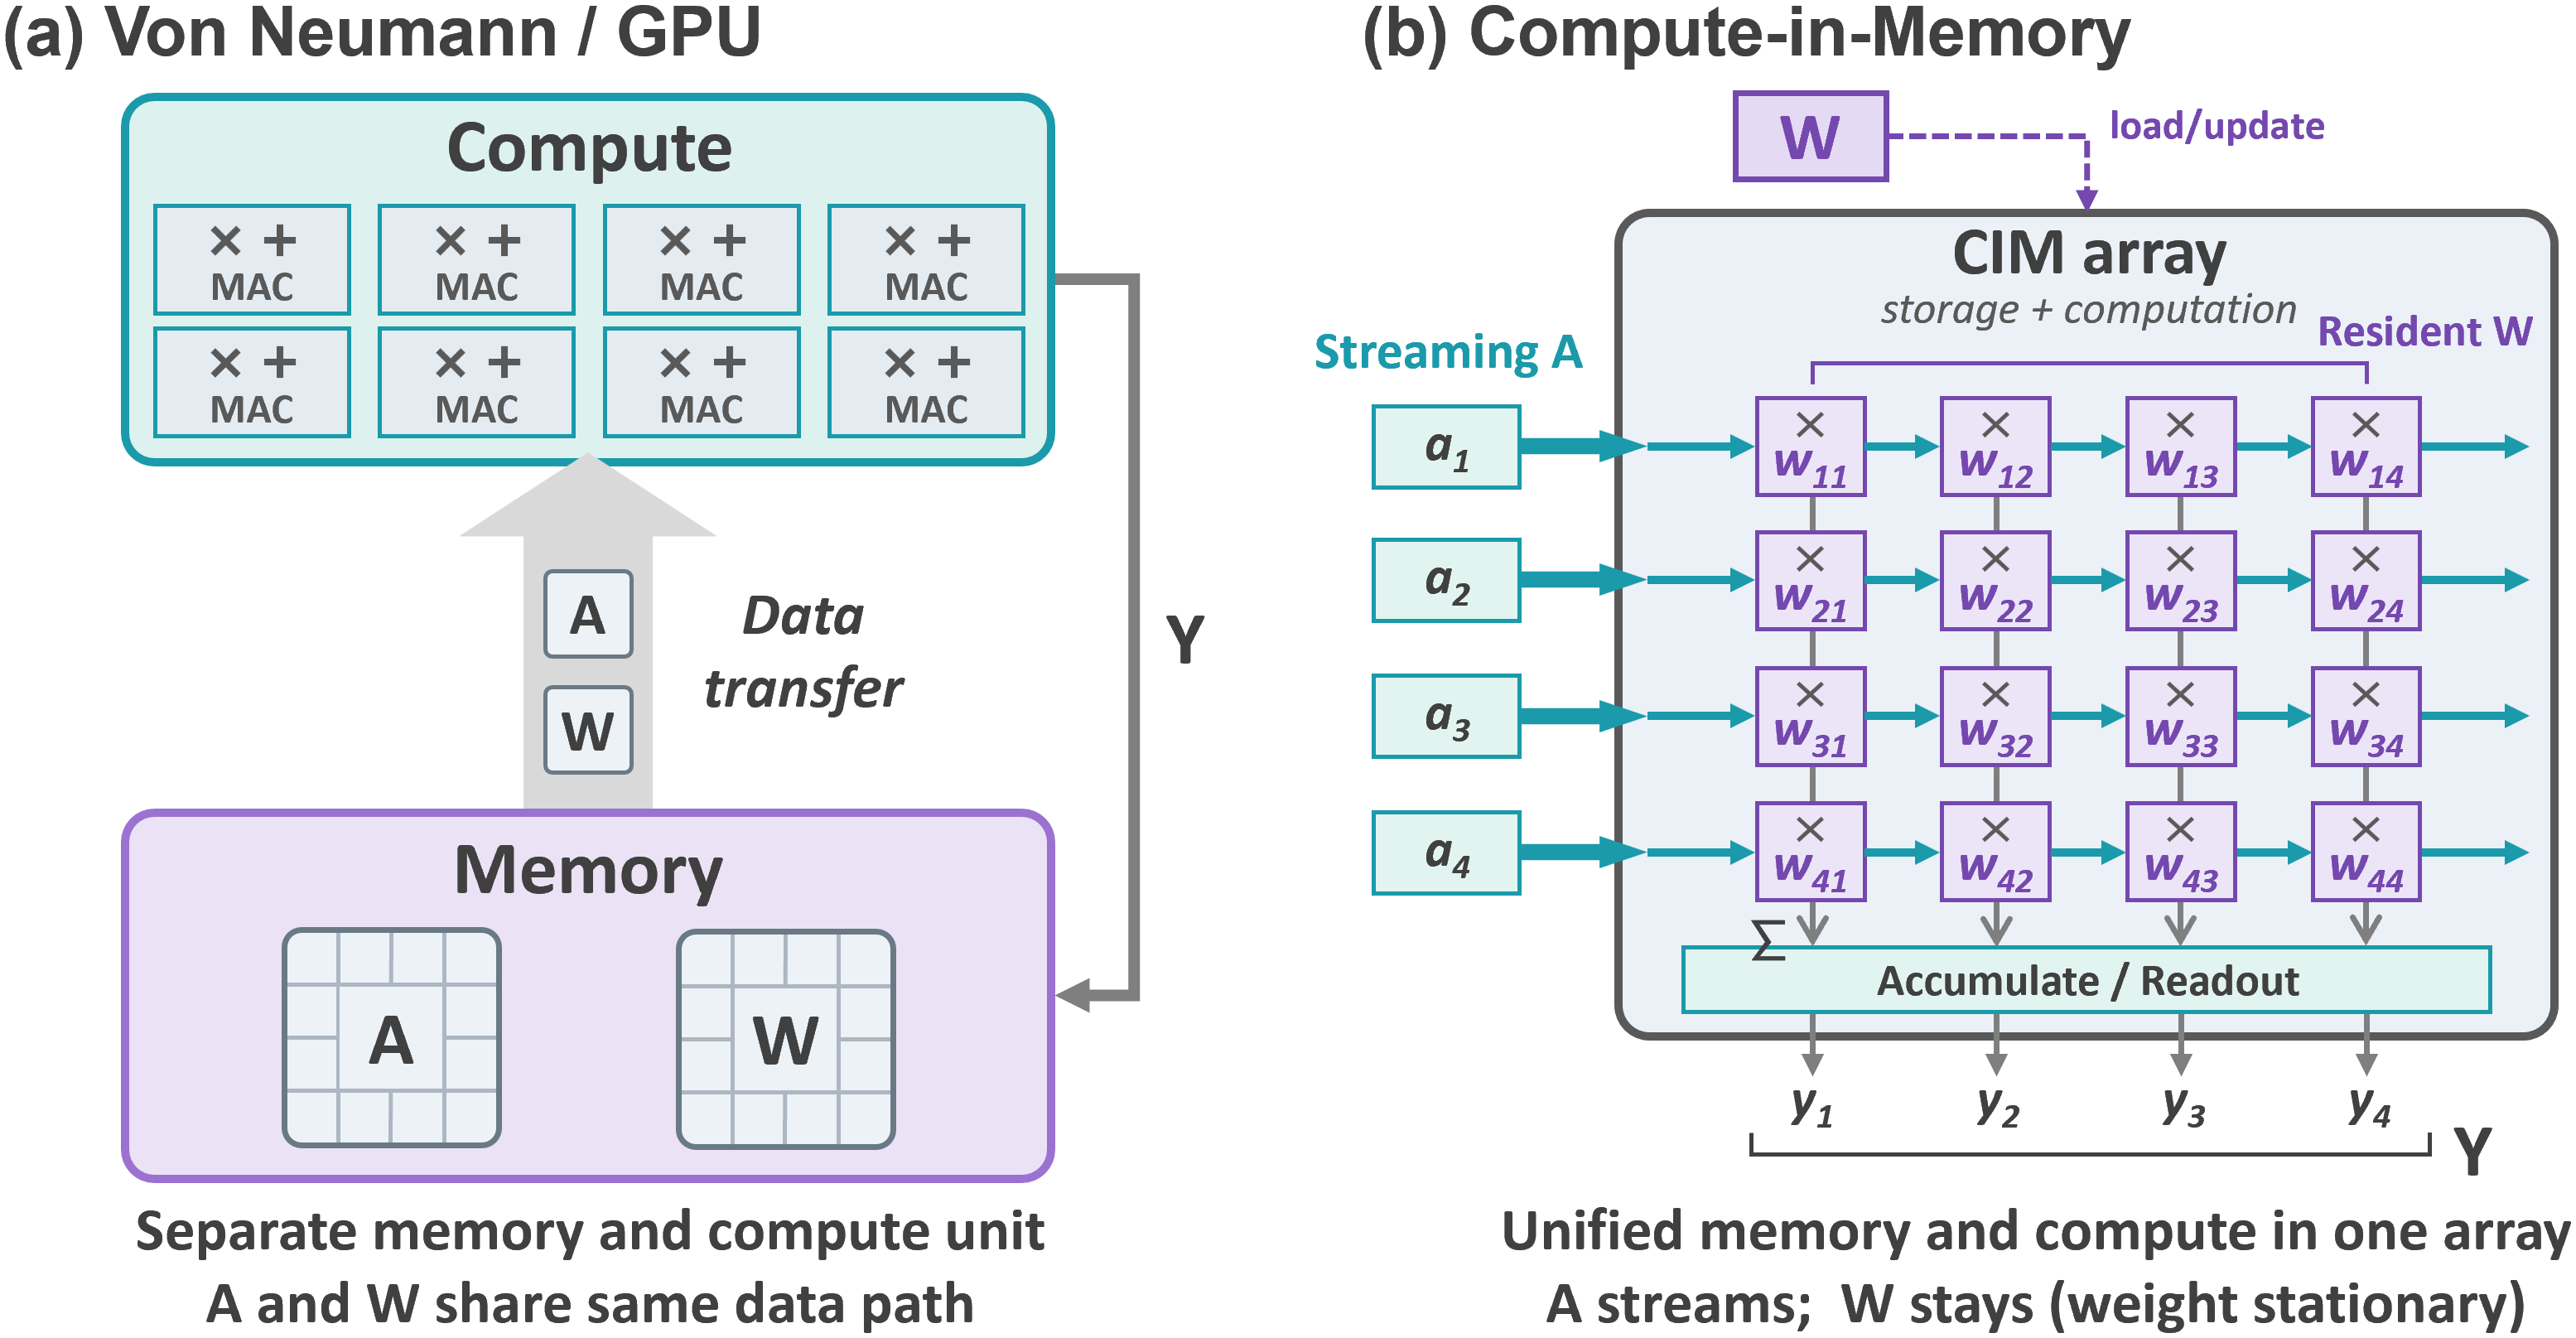
\includegraphics[width=\linewidth]{figures/Fig1_cropped.png}
\caption{Operand roles in (a) separate memory and compute units and (b) a CIM array. Streaming inputs $A$ are evaluated against resident weights $W$, with a distinct path for loading or updating $W$.}
\label{fig:operand-roles}
\vspace{-20pt}
\end{figure}


\section{Proposed Resident-Streaming Roofline}
\label{sec:model}
\subsection{Workload Demands and Hardware Throughputs}
Following the operand roles in Fig.~\ref{fig:operand-roles}(b), the model analyzes a \emph{workload window}, which specifies the input work and the resident state at its start.

Within the window, the streaming demand $Q_S$ is the number of streaming input bytes served at the chosen logical input boundary, and the resident demand $Q_R$ is the number of logical bytes actually written to load, update, or reload resident state. An initial load counts only if it occurs inside the window. The resident operand may be a weight or, in attention, the KV cache of earlier tokens.

Each demand is served by its own throughput. The streaming throughput $\rho$ is the maximum rate at which the hardware serves logical input bytes while completing the specified calculation and outputs. The resident throughput $\tau$ is the maximum rate at which logical resident bytes become ready for calculation under a given write mode. Each demand and its throughput share the same configuration and precision. We define
\begin{equation}
  \SI=\frac{Q_S}{Q_R},\qquad P=\frac{Q_S}{T}\quad[\Byte/\mathrm{s}],
  \label{eq:definitions}
\end{equation}
where $T$ is the window completion time, $P$ is the average streaming-input throughput over the window, and $\SI$ is the streaming demand per byte of resident write, with $\SI=\infty$ for $Q_S>0$ and $Q_R=0$.

Demands count logical bytes; the physical steps that serve them, such as bit-serial cycles, repeated conversions, or program and verify steps, enter the service time of the corresponding path. Maintenance that preserves existing state, such as refresh, also consumes service time but is not a new logical update. A repeated input is counted again only when it re-crosses the chosen boundary, and each demand is paired with the throughput defined at that boundary.

\paperplacefigtwo

\subsection{Throughput Bound and Roofline Interpretation}
Each path imposes a necessary service time on the window: at least $Q_S/\rho$ for streaming and $Q_R/\tau$ for resident writes. The window cannot complete before the longer of the two, and dividing $Q_S$ by this time bounds its throughput:
\begin{align}
  T&\geq\max\!\left(\frac{Q_S}{\rho},\frac{Q_R}{\tau}\right),\label{eq:time}\\
  P&\leq\min(\rho,\tau\SI),\qquad \SI^*=\frac{\rho}{\tau}.
  \label{eq:roofline}
\end{align}
The two service requirements balance at the ridge $\SI^*$. For $\SI<\SI^*$, the resident term is tighter and the window is resident-bound; for $\SI>\SI^*$, the streaming term is tighter and the window is streaming-bound. The bound holds whether or not the two services overlap; shared resources, execution dependencies, and scheduling may keep the actual throughput below it.

Fig.~\ref{fig:roofline-comparison} sets this bound beside the classical Roofline: the demand--throughput pairing is preserved, but work is measured in streaming input bytes rather than operations. Within one execution, $P$ still converts to useful operations per second, $P_{\mathrm{OP}}$: for a logical $128\times128$ INT8 matrix-vector multiplication at two operations per MAC, each input byte corresponds to 256 OP, so $P_{\mathrm{OP}}=(256\ \mathrm{OP}/\Byte)\,P$ for this execution.

\subsection{From Streaming Intensity to Reuse}
The ridge can be expressed as the number of input vectors that one resident load must support. Consider a resident matrix $W[N,K]$ with output dimension $N$ and input dimension $K$, and let the reuse count $U$ be the number of input vectors served after one complete load, including the first use; these vectors may accumulate across batches or requests. With $b_S$ and $b_R$ bytes per streaming and resident element,
\begin{equation}
  Q_S=UKb_S,\qquad Q_R=NKb_R,\qquad \SI=\frac{Ub_S}{Nb_R}.
  \label{eq:matrix-demand}
\end{equation}
At equal byte widths, $\SI=U/N$, as listed for five logical matrices in Table~\ref{tab:reuse-intensity}; for fixed $U$ and precision, $K$ scales both demands equally and cancels.
\paperplacetableone

The same matrix yields different $\SI$ under different residency policies. Reloading before every input fixes $U=1$ per load, however many inputs the window serves. A matrix already resident before the window and never rewritten gives $Q_R=0$, $\SI=\infty$, and $P\leq\rho$; this pre-resident window differs from unbounded reuse after one load, $U\to\infty$, which keeps $Q_R=NKb_R$ finite.

On the hardware side, let $\Delta_S$ be the steady-state service interval of one complete input vector and $T_R$ the service time of one complete load, so that $\rho=Kb_S/\Delta_S$ and $\tau=NKb_R/T_R$. Setting $\SI=\SI^*$ gives the \emph{critical reuse}
\begin{equation}
  U^*=\frac{T_R}{\Delta_S}=\frac{Nb_R}{b_S}\,\SI^*,
  \label{eq:critical-reuse}
\end{equation}
which reduces to $U^*=N\SI^*$ at equal byte widths. The two service requirements thus balance at $U\Delta_S=T_R$: serving $U^*$ input vectors takes as much service time as one complete load. A load-once window is therefore resident-bound for $U<U^*$ and streaming-bound for $U>U^*$. Here, $U$ is the reuse a workload offers, whereas $U^*$ is the reuse the hardware requires, set by its load time relative to its input service interval.

For this load-once reference, normalizing~\eqref{eq:roofline} by $\rho$ gives
\begin{equation}
  \frac{P}{\rho}\leq\min\!\left(1,\frac{\SI}{\SI^*}\right)=\min\!\left(1,\frac{U}{U^*}\right),
  \label{eq:reuse-bound}
\end{equation}
so insufficient reuse caps the throughput at a fraction $U/U^*$ of the streaming ceiling.

\draftspread{%
  \begin{paperwidefigure}
% Submission typography; original vector and all geometry retained separately.
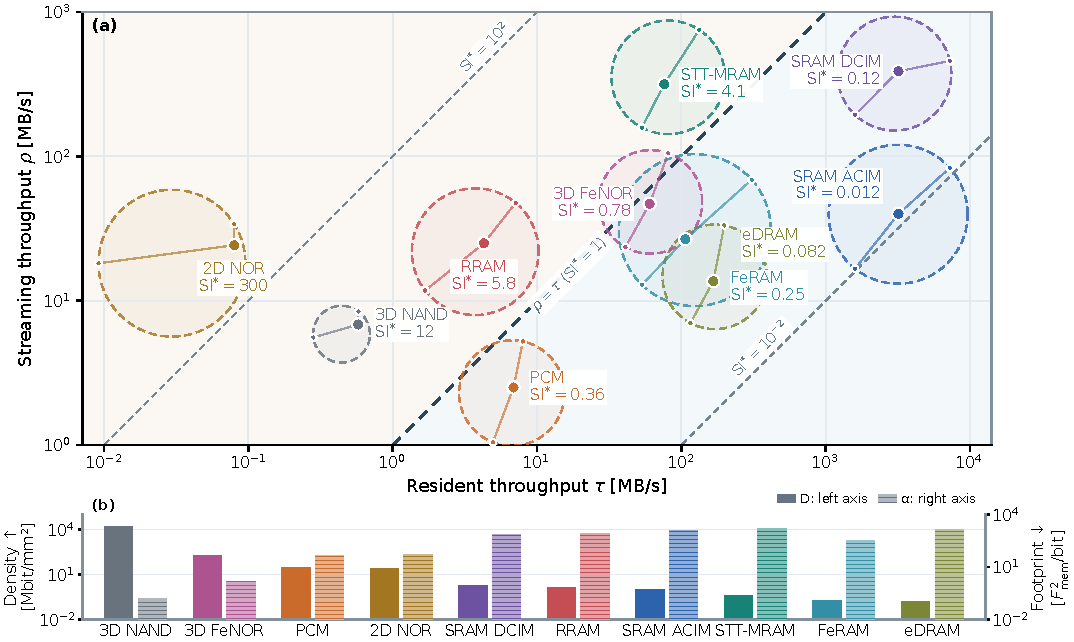
\includegraphics[width=\textwidth]{figures/hardware_capacities_paper.pdf}
\caption{Streaming capacity $\rho$ and resident-update capacity $\tau$ for ten native reference configurations; $1\ \mathrm{MB/s}=10^6\ \Byte/\mathrm{s}$. Large points are typical scenarios; small points preserve the original paired alternatives. Circles summarize only those finite scenarios, and $\RI^*=1$ is a capacity-ratio reference, not a universal workload boundary. Native sizes and resources differ.}
\label{fig:hardware-capacities}
\end{paperwidefigure}

  \par\medskip
  % Selected from Task II(b) 04_crosscheck/data/results.json; no O-projection values are implied.
\begin{paperwidetable}
\caption{Streaming intensities of representative inference matrix stages}
\label{tab:workload-intensity}
\footnotesize\setlength{\tabcolsep}{1.6pt}\renewcommand{\arraystretch}{1.25}
\begin{tabularx}{\textwidth}{@{}p{0.20\textwidth}*{12}{>{\centering\arraybackslash}X}@{}}
\toprule
& \multicolumn{6}{c}{\textbf{Weight projections}} & \multicolumn{6}{c}{\textbf{Attention}} \\
\cmidrule(lr){2-7}\cmidrule(l){8-13}
& \multicolumn{3}{c}{QKV ($U$)} & \multicolumn{3}{c}{FFN/MoE ($U$)} & \multicolumn{3}{c}{Prefill ($L$)} & \multicolumn{3}{c}{Decode ($L$)} \\
\cmidrule(lr){2-4}\cmidrule(lr){5-7}\cmidrule(lr){8-10}\cmidrule(l){11-13}
Model & $1\Kilo$ & $128\Kilo$ & $1\mathrm{M}$ & $16$ & $1\Kilo$ & $16\Kilo$ & $1\Kilo$ & $8\Kilo$ & $64\Kilo$ & $1\Kilo$ & $8\Kilo$ & $64\Kilo$ \\
\midrule
Qwen3.5-2B & 0.200 & 25.6 & 204.8 & 0.00347 & 0.222 & 3.6 & 6.0 & 34.0 & 258.0 & 10.0 & 66.0 & 514.0 \\
Ministral 3 8B & 0.167 & 21.3 & 170.7 & 0.00167 & 0.107 & 1.7 & 10.0 & 66.0 & 514.0 & 18.0 & 130.0 & 1026.0 \\
Qwen3.6-35B-A3B & 0.111 & 14.2 & 113.8 & 0.0130 & 0.833 & 13.3 & 12.0 & 68.0 & 516.0 & 20.0 & 132.0 & 1028.0 \\
Hy3 (295B) & 0.100 & 12.8 & 102.4 & 0.00477 & 0.306 & 4.9 & 20.0 & 132.0 & 1028.0 & 36.0 & 260.0 & 2052.0 \\
Ling-1T (1000B) & 0.100 & 12.8 & 102.4 & 0.00326 & 0.208 & 3.3 & 20.0 & 132.0 & 1028.0 & 36.0 & 260.0 & 2052.0 \\
MiMo-V2.5-Pro (1020B) & 0.0377 & 4.8 & 38.6 & 0.00347 & 0.222 & 3.6 & 35.2 & 214.4 & 1648.0 & 60.8 & 419.2 & 3286.4 \\
\bottomrule\end{tabularx}
\par\smallskip\raggedright
Entries are $\SI$; all roles use one byte/element. QKV includes any gate, excluding O. FFN/MoE counts one dense FFN or one routed expert. Prefill builds KV from empty; decode appends one token to a visible length $L$. $1\Kilo=1024$, $1\mathrm{M}=1024^2$. Ling-1T at $64\Kilo$ uses the fixed extension.
\end{paperwidetable}

}
\section{Hardware and Workload Characterization}
\label{sec:characterization}
\subsection{Memory-Based Reference Configurations}
\outline{Introduce the ten native analog/digital reference configurations in Fig.~\ref{fig:hardware-capacities}, grounded in device and macro sources~\cite{SACIM-03,SDCIM-01,NOR-01,NAND-05,RRAM-01,MRAM-06,PCM-01,FERAM-01,GC-04,FENOR-02} and shared peripheral assumptions~\cite{CMOS-02,CMOS-03,CMOS-07}. Explain the three paired engineering scenarios and complete service accounting, retaining native matrix dimensions, resources, and update organizations. Read absolute capacity and capacity ratio separately; these are literature-grounded estimates rather than equal-area chip comparisons.}
\draftreserve{0.35in}{Native configurations and complete service accounting.}
\draftcolumnbreak
\subsection{Inference Matrix Workloads}
\outline{Use the six fixed model configurations~\cite{qwen35,ministral3,qwen36,hy3,ling,mimo} as structural examples for Table~\ref{tab:workload-intensity}, counting common inputs once per matrix stage at one byte per element. Explain QKV intensity $U/N_{\mathrm{proj}}$ and FFN intensity $U(D+F)/(3DF)$ using output width $N_{\mathrm{proj}}$ (including any gate), hidden width $D$, and dense-FFN or single-expert width $F$. For grouped-query attention, use the native head sharing and possibly unequal query/key and value widths: prefill creates each token's KV once, whereas decode appends one token and treats historical KV as resident.}

\draftpagebreak
\section{Reuse Requirements and Design Implications}
\label{sec:implications}
\subsection{Critical Reuse Across Configurations}
\outline{Use Fig.~\ref{fig:critical-reuse} to show that typical full-load thresholds span about 1.6 to 38,867 input vectors, then develop one concrete crossing: at the illustrative reuse $U=128$, STT-MRAM is resident-bound in the short and typical scenarios (about 181 and 133), but streaming-bound in the long scenario (about 95). Connect the native threshold to Qwen3.5-2B and MiMo-V2.5-Pro QKV stages using the existing sequential full-tile service reference, for which both sides accumulate the same tile count. Keep this mapping as a component-service bound, with output reduction and other system costs outside its scope.}

For native $128\times128$ tiles, let $m_K=D/128$, $m_N=N_{\mathrm{proj}}/128$, and $M=m_Km_N$:
\begin{align}
 T_{S,\mathrm{comp}}&=MU\Delta_S,&
 T_{R,\mathrm{comp}}&=MT_R,\label{eq:tile-times}\\
 \rho_{\mathrm{eff}}&=\rho/m_N,&
 \tau_{\mathrm{eff}}&=\tau,\label{eq:effective-capacity}\\
 \SI^*_{\mathrm{eff}}&=\frac{\SI^*}{m_N}=\frac{U^*}{N_{\mathrm{proj}}}.
 \label{eq:effective-ridge}
\end{align}
The factor $M$ cancels at service balance. This reference uses one engine, full tiles without padding, and equal $U$ per tile; input replay is included in $T_{S,\mathrm{comp}}$.
\draftreserve{0.65in}{Explain the threshold span and one scenario crossing.}
\draftcolumnbreak
\begin{paperfigure}
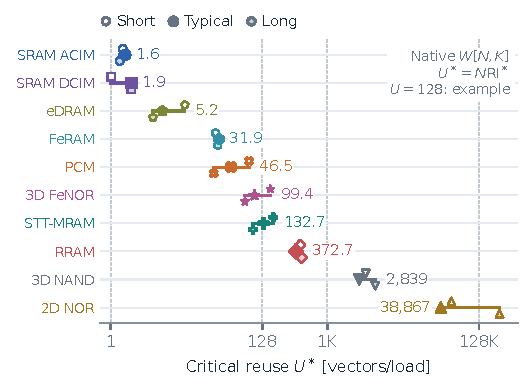
\includegraphics[width=\columnwidth]{figures/critical_reuse_single.pdf}
\caption{Full-load critical reuse $U^*=T_R/\Delta_S=N\SI^*$ at equal byte widths; each row uses its native $W[N,K]$. Numbers give typical values; segments span only three paired scenarios. Dashed lines mark illustrative reuse counts, not universal balance points. $1\Kilo=1024$.}
\label{fig:critical-reuse}
\end{paperfigure}

\subsection{Design Implications}
\outline{Turn a target reuse count into an allowable full-load service time using \eqref{eq:load-budget}, making Fig.~\ref{fig:critical-reuse} a design requirement rather than a ranking. Revisit Fig.~\ref{fig:hardware-capacities} to explain why a lower threshold alone does not imply higher performance: streaming throughput still sets the upper plateau. Contrast weight residency with growing attention state in Table~\ref{tab:workload-intensity}; KV append requires its own update-service boundary before applying any full-load threshold.}
\begin{equation}
  T_R\leq U_{\mathrm{target}}\Delta_S
  \quad\Longleftrightarrow\quad U_{\mathrm{target}}\geq U^*.
  \label{eq:load-budget}
\end{equation}
This is a necessary service-balance condition for reaching the streaming ceiling, not a guarantee of realized throughput.
\draftreserve{0.75in}{Turn a target reuse count into a resident-service requirement.}

\section{Conclusion}
\outline{Close with the role-based connection between in-window resident updates and streaming evaluation established by \eqref{eq:roofline}. Use Fig.~\ref{fig:critical-reuse} to emphasize the practical outcome: hardware service asymmetry becomes an explicit reuse requirement for residency and update decisions.}
\draftreserve{0.45in}{Final conclusion: one short paragraph.}


% Flush every body float before the real, fifth physical page.
\clearpage
\iflayoutdraft\IEEEtriggeratref{12}\fi
\bibliographystyle{IEEEtran}
\bibliography{references}
\end{document}
